\section{Implications for Higgs and weak boson production}
\label{sec:pheno}

The reduction of PDF uncertainties made possible by neutrino DIS measurements
at the FPF, discussed in Sect.~\ref{sec:protonPDFs},
enables more precise theoretical predictions for core processes at the
HL-LHC.
%
Here we present an initial study of the phenomenological implications
of the PDFs enhanced with LHC neutrino data
for hard-scattering processes at proton colliders.
%
Specifically, we present results for 
single and double gauge boson production,  Higgs production in
vector-boson fusion, and Higgs production and in association with a vector boson.
%
We focus on processes sensitive to the quark-quark and quark-antiquark initial
states, given that LHC neutrinos do not provide information on the gluon
PDF and hence they cannot inform  gluon-initiated
processes, such as top quark pair production or Higgs production in gluon fusion.

We adopt the same calculational settings as in the LHC phenomenology analysis considered
in the PDF4LHC21 combination study~\cite{PDF4LHCWorkingGroup:2022cjn} and provide predictions
both for inclusive cross-sections, integrated in the fiducial
region, and for differential distributions.
%
We evaluate these cross-sections using matrix elements
which include NLO corrections both in the
QCD and electroweak coupling using
{\sc\small mg5\_amc@nlo}~\cite{Frederix:2018nkq}
interfaced to {\sc\small PineAPPL}~\cite{Carrazza:2020gss}.
%
For all processes, realistic selection and acceptance cuts on the final state particles
have been applied.
%
No further theory uncertainties are considered in this
analysis, given that we don't aim to compare with experimental data.

Fig.~\ref{fig:NNPDF40_pheno_integrated} displays
fiducial cross-section for representative LHC processes at $\sqrt{s}=14$ TeV
evaluated with NNPDF4.0 (top panels)
and with PDF4LHC21 (bottom panels),
compared with the results obtained from
the fits including the FPF structure function projections.
%
For the latter, we display the variants based only on statistical uncertainties and that
which includes also systematic errors.
%
The central values are set to be the same as in the original NNPDF4.0 calculation in all cases.
%
See~\cite{NNPDF:2021njg} for the calculational settings.
%
From top to bottom, we show inclusive Drell-Yan production ($Z, W^+, W^-$), Higgs production
in vector-boson fusion, Higgs associated
production, and diboson production ($W^+W^-$, $W^+Z$, $W^-Z$).
%
The corresponding comparison at the level of differential distributions
are shown in Fig.~\ref{fig:NNPDF40_pheno_differential}.
%
As done for the fiducial cross-sections of Fig.~\ref{fig:NNPDF40_pheno_integrated},
we only indicate the relative PDF uncertainty in each fit, with central values
assumed to be the same by construction.


%%%%%%%%%%%%%%%%%%%%%%%%%%%%%%%%%%%%%%%%%%%%%%%%%%%%%%%%%%%%%%%%%%%%%%%%
\begin{figure}[htbp]
\centering
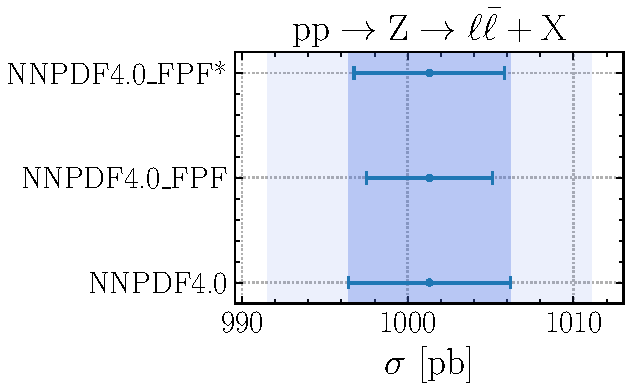
\includegraphics[width=0.32\textwidth]{plots/LHCpheno/NNPDF_DY_14TEV_40_PHENO-integrated.pdf}
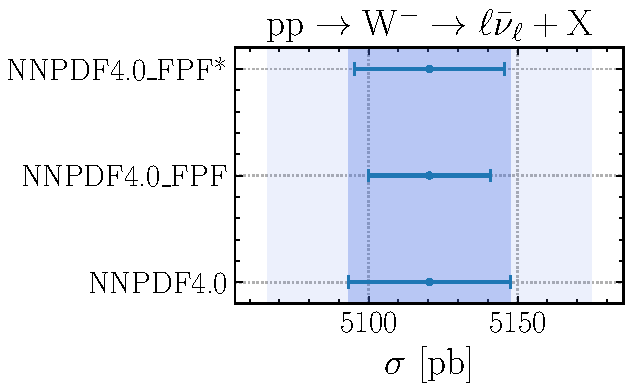
\includegraphics[width=0.32\textwidth]{plots/LHCpheno/NNPDF_WM_14TEV_40_PHENO-integrated.pdf}
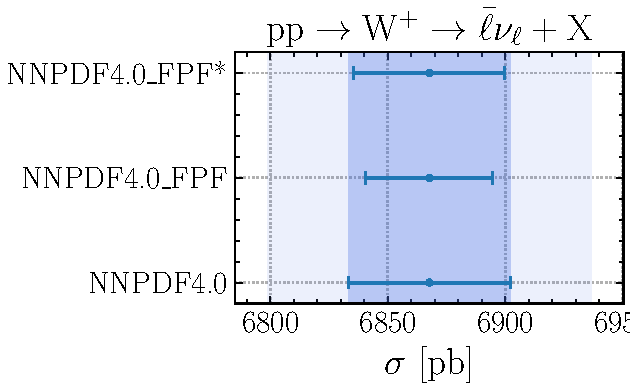
\includegraphics[width=0.32\textwidth]{plots/LHCpheno/NNPDF_WP_14TEV_40_PHENO-integrated.pdf}
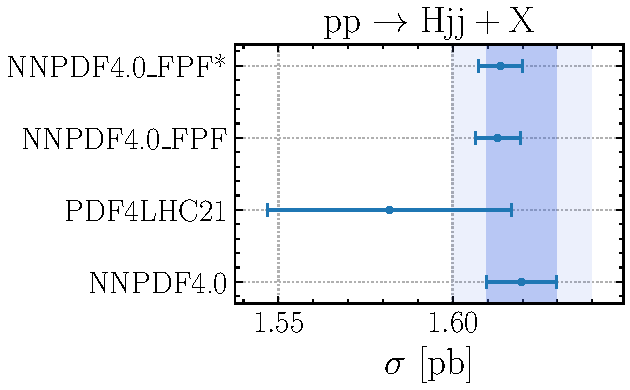
\includegraphics[width=0.32\textwidth]{plots/LHCpheno/NNPDF_HVBF_14TEV_40_PHENO-integrated.pdf}
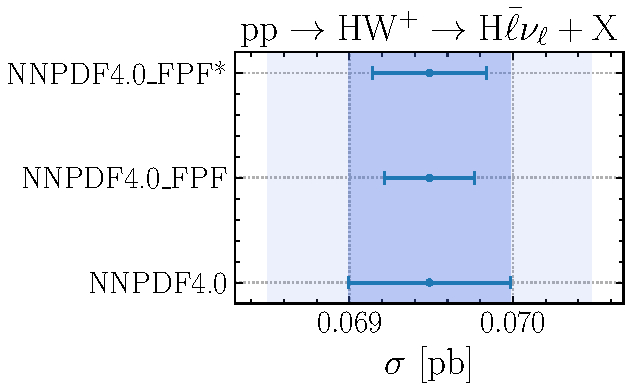
\includegraphics[width=0.32\textwidth]{plots/LHCpheno/NNPDF_HWP_14TEV_40_PHENO-integrated.pdf}
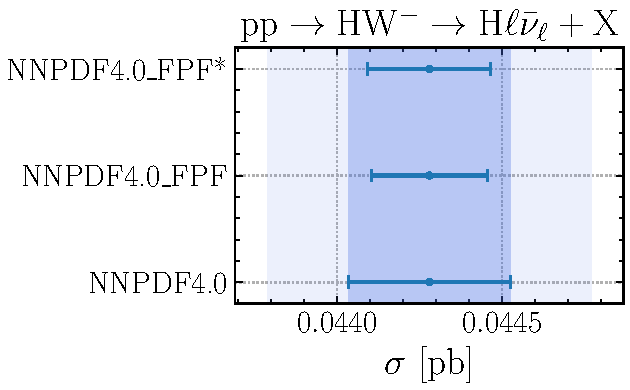
\includegraphics[width=0.32\textwidth]{plots/LHCpheno/NNPDF_HWM_14TEV_40_PHENO-integrated.pdf}
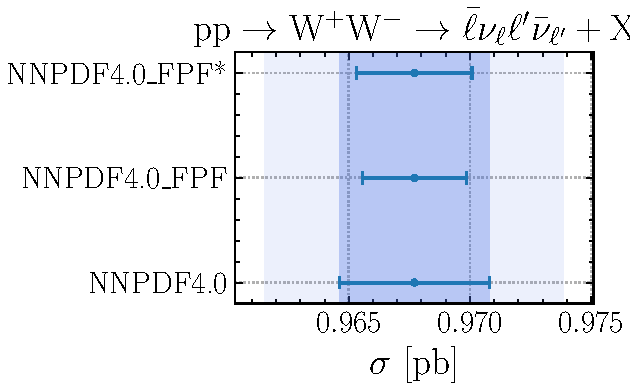
\includegraphics[width=0.32\textwidth]{plots/LHCpheno/NNPDF_WPWM_14TEV_40_PHENO-integrated.pdf}
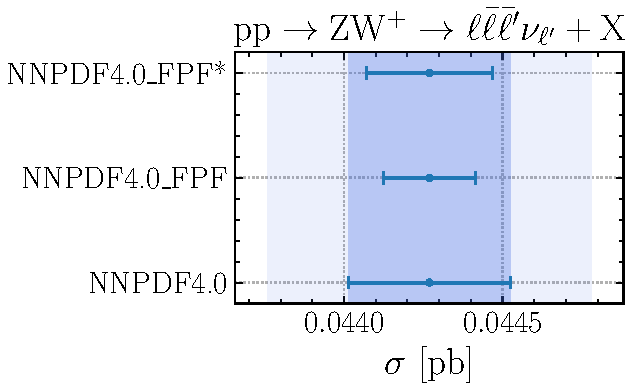
\includegraphics[width=0.32\textwidth]{plots/LHCpheno/NNPDF_WPZ_14TEV_40_PHENO-integrated.pdf}
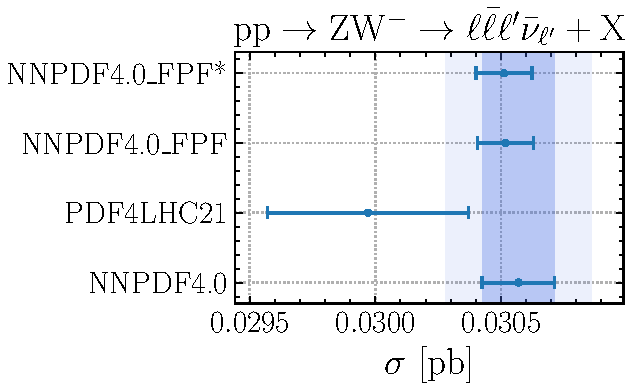
\includegraphics[width=0.32\textwidth]{plots/LHCpheno/NNPDF_WMZ_14TEV_40_PHENO-integrated.pdf}
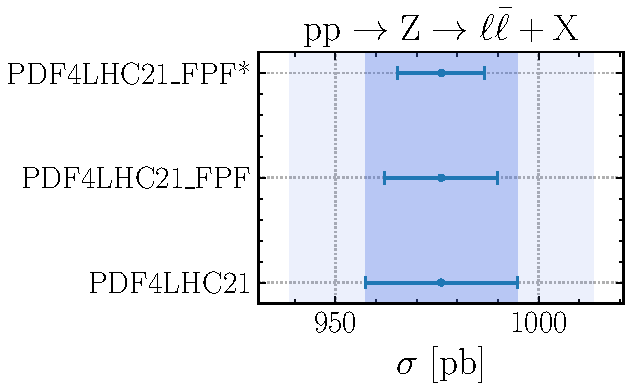
\includegraphics[width=0.32\textwidth]{plots/LHCpheno/NNPDF_DY_14TEV_40_PHENO-integrated-pdf4lhc21.pdf}
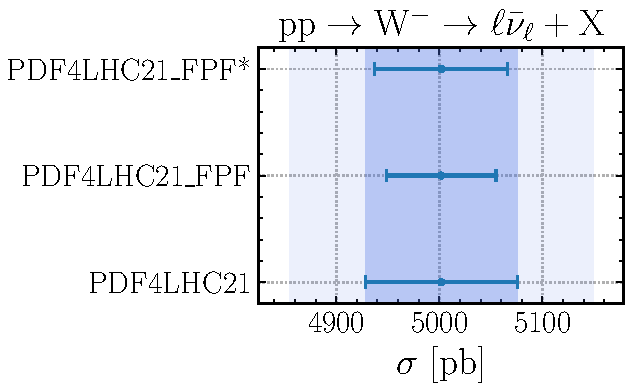
\includegraphics[width=0.32\textwidth]{plots/LHCpheno/NNPDF_WM_14TEV_40_PHENO-integrated-pdf4lhc21.pdf}
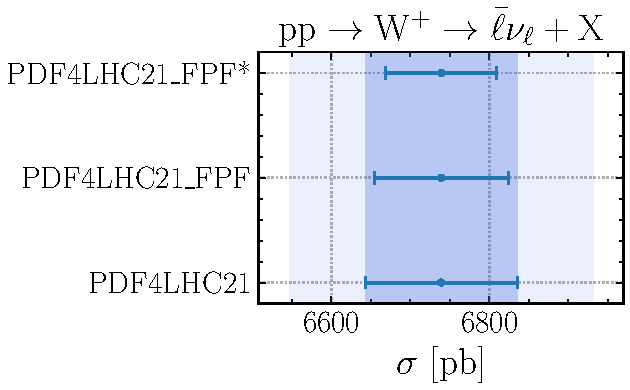
\includegraphics[width=0.32\textwidth]{plots/LHCpheno/NNPDF_WP_14TEV_40_PHENO-integrated-pdf4lhc21.pdf}
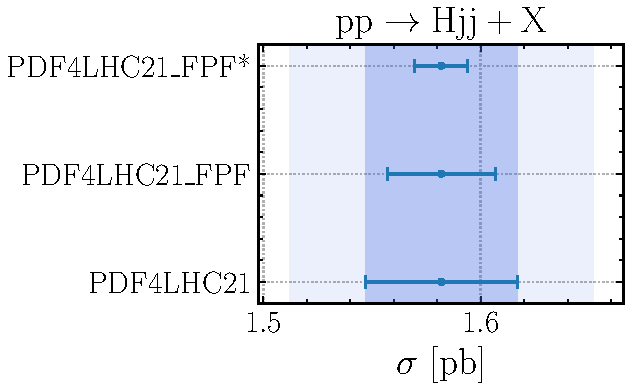
\includegraphics[width=0.32\textwidth]{plots/LHCpheno/NNPDF_HVBF_14TEV_40_PHENO-integrated-pdf4lhc21.pdf}
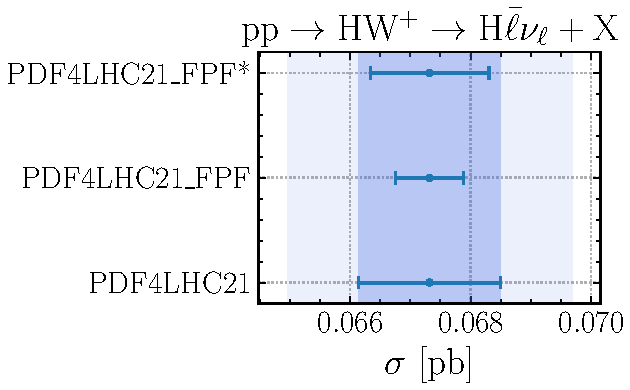
\includegraphics[width=0.32\textwidth]{plots/LHCpheno/NNPDF_HWP_14TEV_40_PHENO-integrated-pdf4lhc21.pdf}
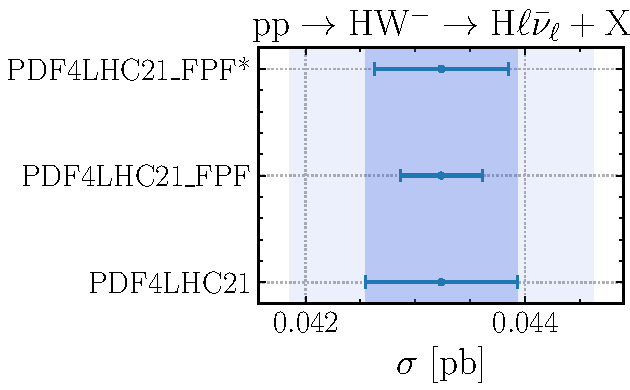
\includegraphics[width=0.32\textwidth]{plots/LHCpheno/NNPDF_HWM_14TEV_40_PHENO-integrated-pdf4lhc21.pdf}
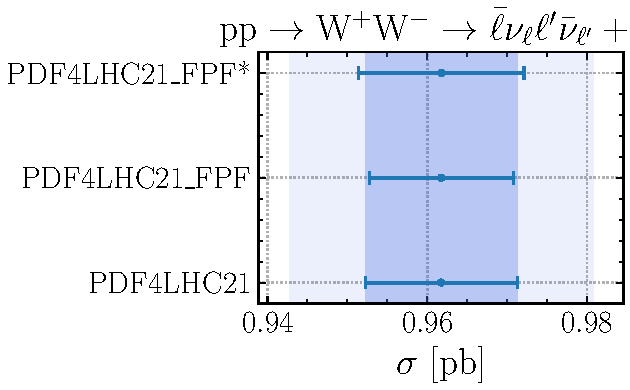
\includegraphics[width=0.32\textwidth]{plots/LHCpheno/NNPDF_WPWM_14TEV_40_PHENO-integrated-pdf4lhc21.pdf}
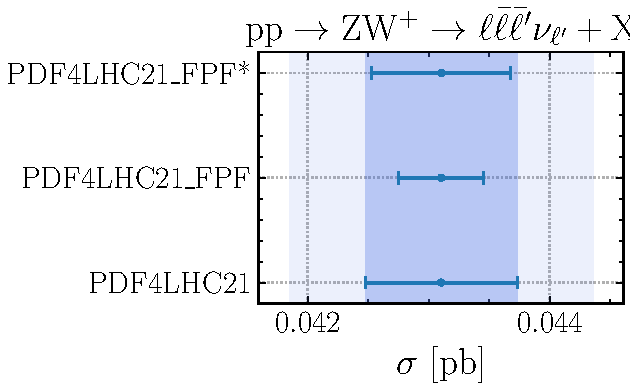
\includegraphics[width=0.32\textwidth]{plots/LHCpheno/NNPDF_WPZ_14TEV_40_PHENO-integrated-pdf4lhc21.pdf}
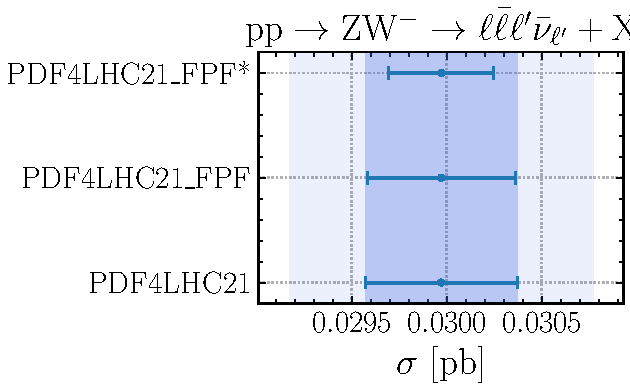
\includegraphics[width=0.32\textwidth]{plots/LHCpheno/NNPDF_WMZ_14TEV_40_PHENO-integrated-pdf4lhc21.pdf}
\caption{Fiducial cross-sections for representative LHC processes at $\sqrt{s}=14$ TeV
  evaluated with NNPDF4.0 (upper panels) and PDF4LHC21 (bottom panels),
  compared with the fits including the FPF structure function projections.
  %
  See~\cite{NNPDF:2021njg,PDF4LHCWorkingGroup:2022cjn} for the calculational settings
  used to evaluate these cross-sections.
%
For the baseline
predictions, the dark (light) bands indicate the 68\% (95\%) CL uncertainties.
%
The fits labelled as ``\_FPF'' are the ones considering statistical uncertainties,
while those labelled as ``\_FPF$^*$'' also include systematic errors.
%
In the fits with FPF data, the central values are set to be the same as
in the corresponding baseline.
%
We provide predictions for inclusive Drell-Yan production ($Z, W^+, W^-$), Higgs production
in vector-boson fusion, Higgs associated
production, and diboson production ($W^+W^-$, $W^+Z$, $W^-Z$).
%
}
\label{fig:NNPDF40_pheno_integrated}
\end{figure}
%%%%%%%%%%%%%%%%%%%%%%%%%%%%%%%%%%%%%%%%%%%%%%%%%%%%%%%%%%%%%%%%%%%%%%%%


%%%%%%%%%%%%%%%%%%%%%%%%%%%%%%%%%%%%%%%%%%%%%%%%%%%%%%%%%%%%%%%%%%%%%%%%
\begin{figure}[htbp]
\centering
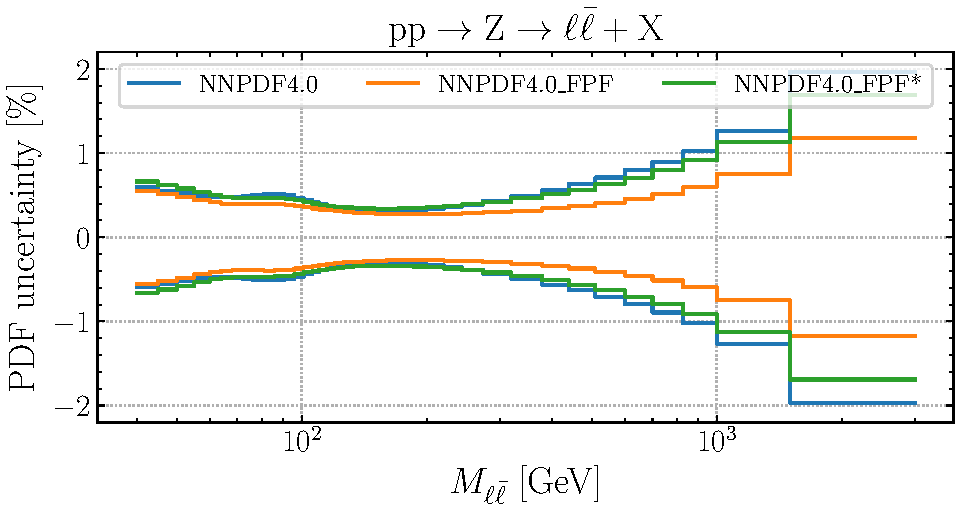
\includegraphics[width=0.49\textwidth]{plots/LHCpheno/NNPDF_DY_14TEV_40_PHENO-global.pdf}
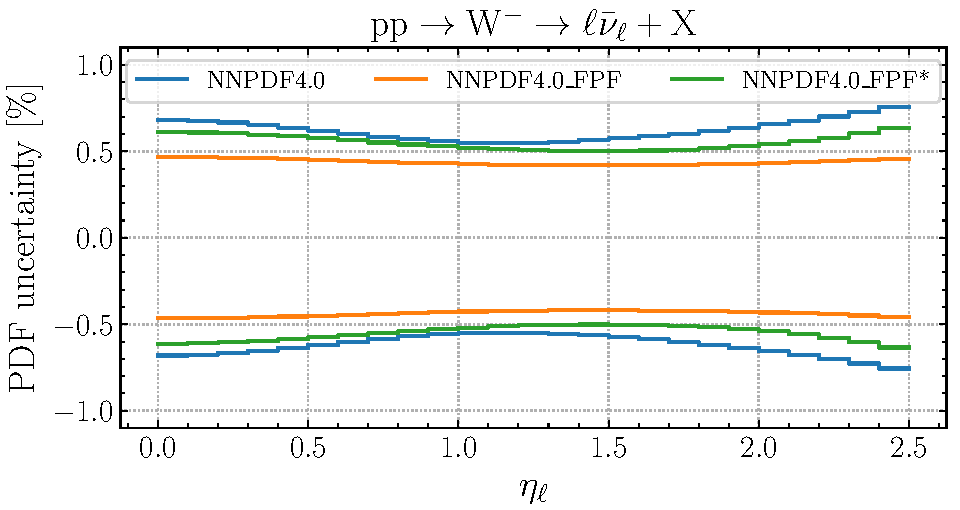
\includegraphics[width=0.49\textwidth]{plots/LHCpheno/NNPDF_WM_14TEV_40_PHENO-global.pdf}
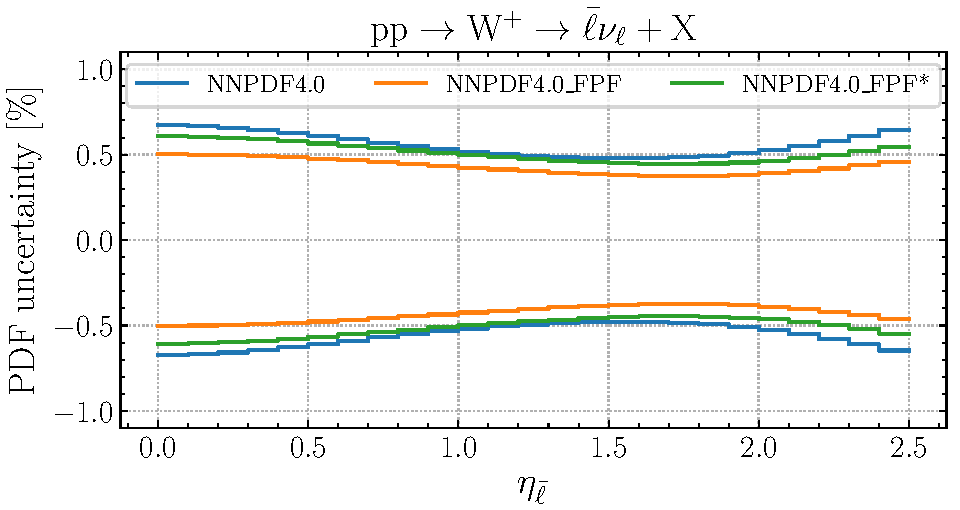
\includegraphics[width=0.49\textwidth]{plots/LHCpheno/NNPDF_WP_14TEV_40_PHENO-global.pdf}
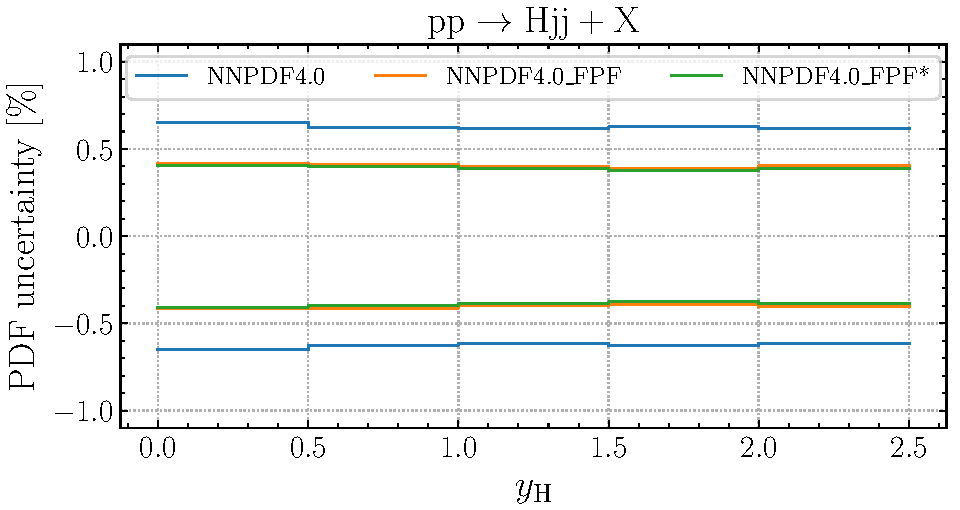
\includegraphics[width=0.49\textwidth]{plots/LHCpheno/NNPDF_HVBF_14TEV_40_PHENO-global.pdf}
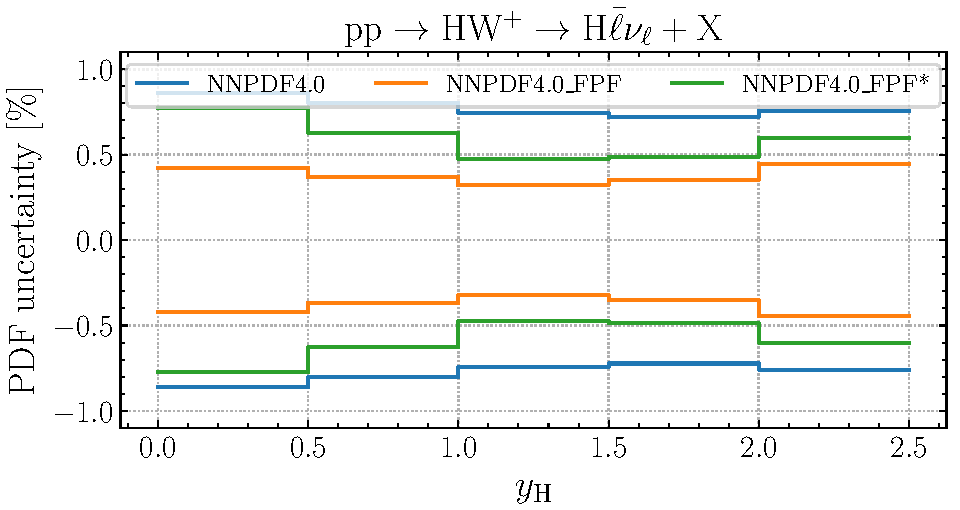
\includegraphics[width=0.49\textwidth]{plots/LHCpheno/NNPDF_HWP_14TEV_40_PHENO-global.pdf}
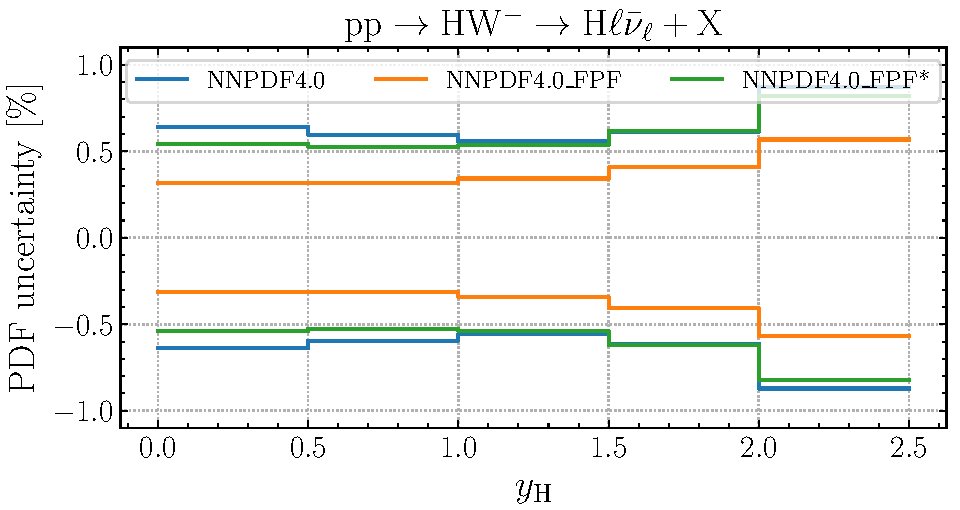
\includegraphics[width=0.49\textwidth]{plots/LHCpheno/NNPDF_HWM_14TEV_40_PHENO-global.pdf}
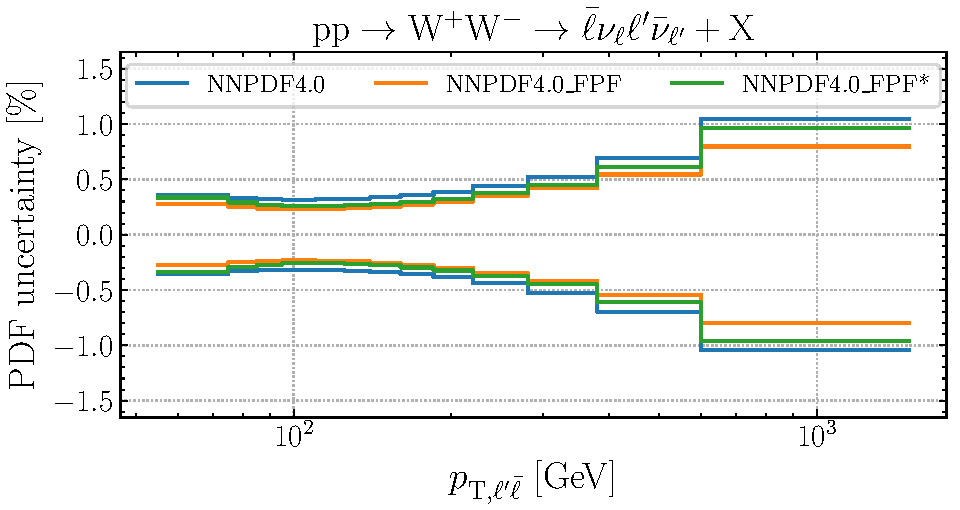
\includegraphics[width=0.49\textwidth]{plots/LHCpheno/NNPDF_WPWM_14TEV_40_PHENO-global.pdf}
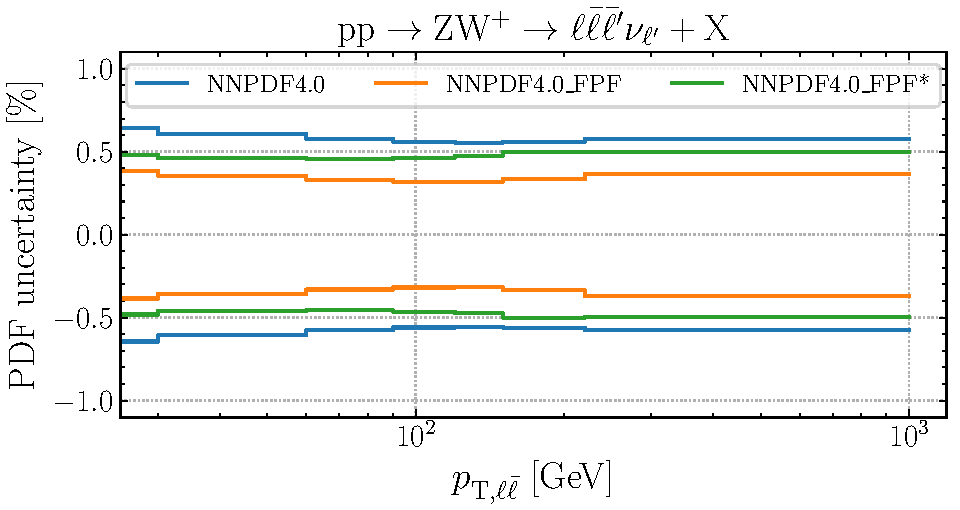
\includegraphics[width=0.49\textwidth]{plots/LHCpheno/NNPDF_WPZ_14TEV_40_PHENO-global.pdf}
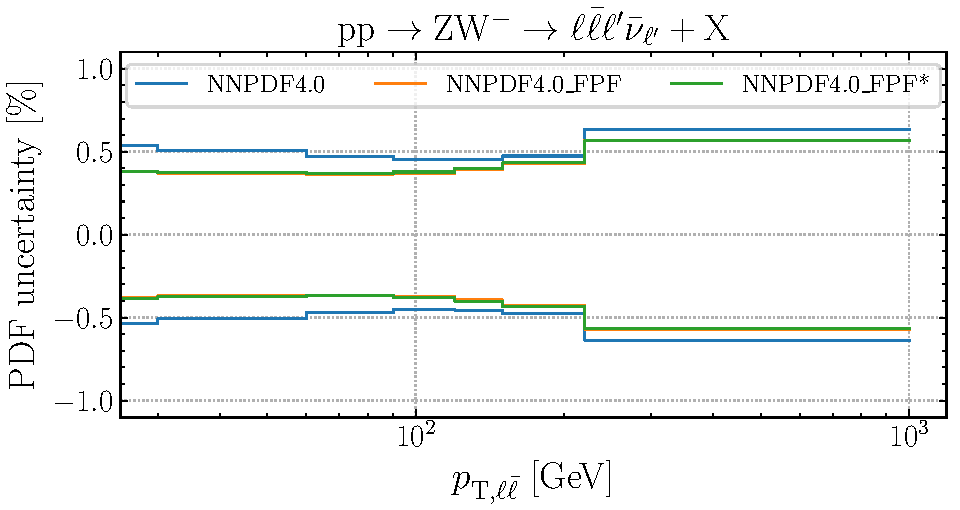
\includegraphics[width=0.49\textwidth]{plots/LHCpheno/NNPDF_WMZ_14TEV_40_PHENO-global.pdf}
\caption{Same as Fig.~\ref{fig:NNPDF40_pheno_integrated}
for the corresponding differential distributions in the case of NNPDF4.0
%
}
\label{fig:NNPDF40_pheno_differential}
\end{figure}
%%%%%%%%%%%%%%%%%%%%%%%%%%%%%%%%%%%%%%%%%%%%%%%%%%%%%%%%%%%%%%%%%%%%%%%%

%%%%%%%%%%%%%%%%%%%%%%%%%%%%%%%%%%%%%%%%%%%%%%%%%%%%%%%%%%%%%%%%%%%%%%%%
\begin{figure}[htbp]
	\centering
	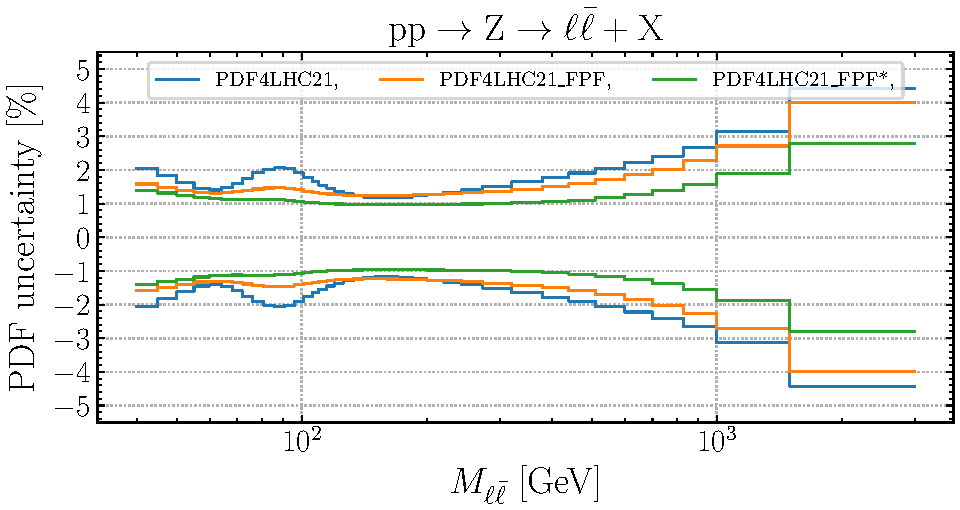
\includegraphics[width=0.49\textwidth]{plots/LHCpheno/NNPDF_DY_14TEV_40_PHENO-global-pdf4lhc21.pdf}
	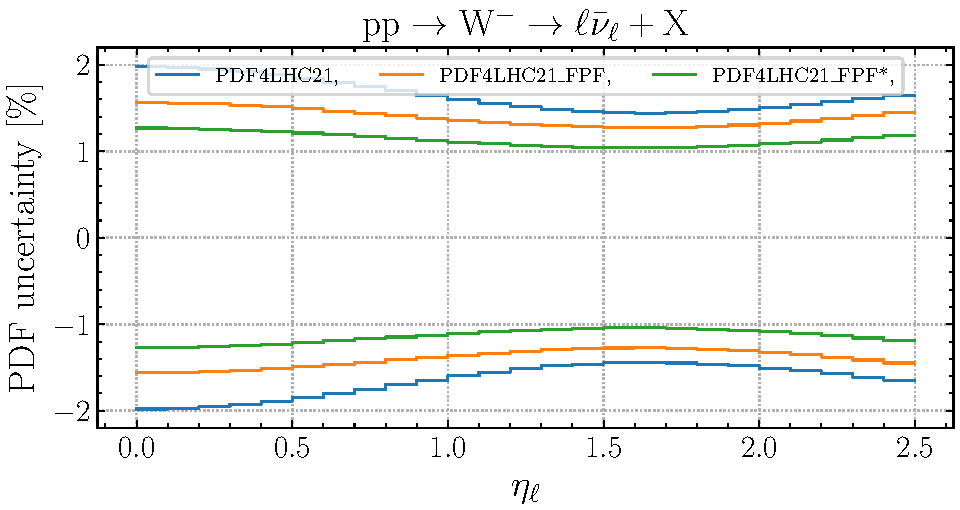
\includegraphics[width=0.49\textwidth]{plots/LHCpheno/NNPDF_WM_14TEV_40_PHENO-global-pdf4lhc21.pdf}
	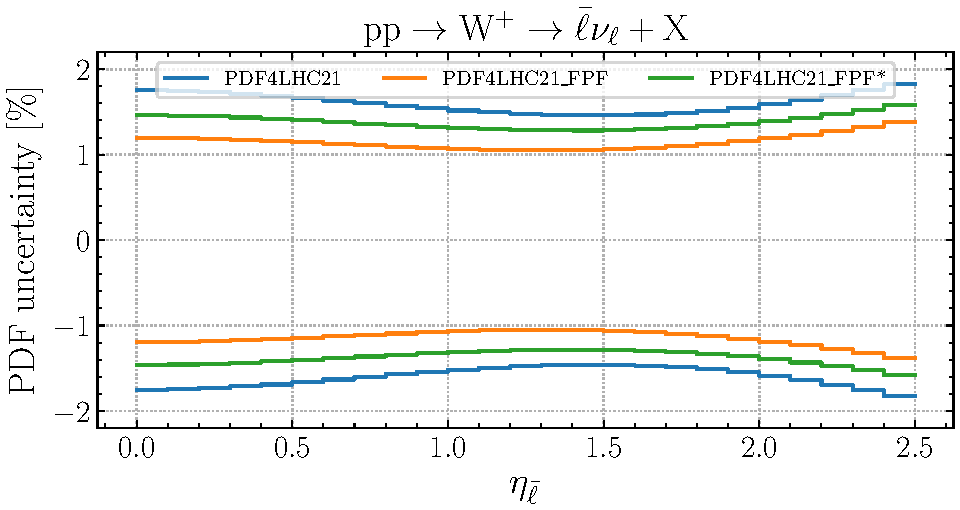
\includegraphics[width=0.49\textwidth]{plots/LHCpheno/NNPDF_WP_14TEV_40_PHENO-global-pdf4lhc21.pdf}
	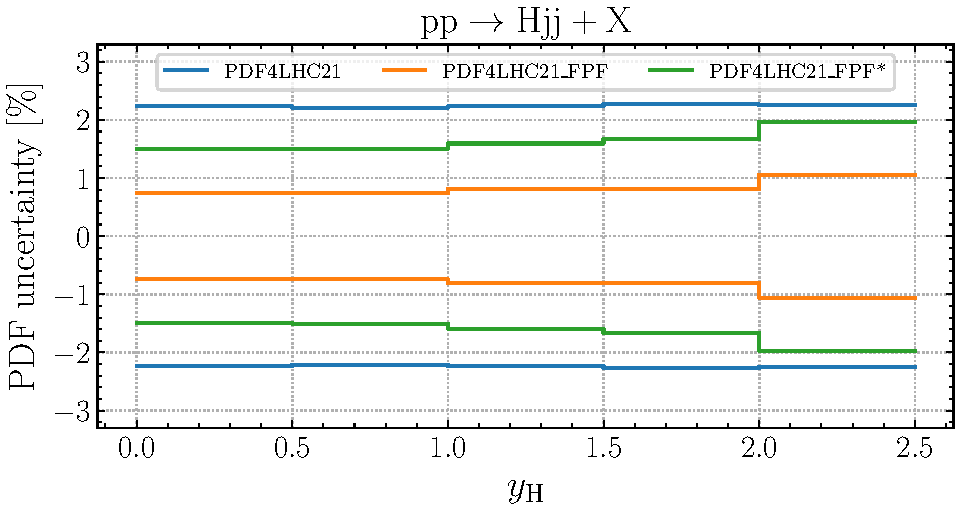
\includegraphics[width=0.49\textwidth]{plots/LHCpheno/NNPDF_HVBF_14TEV_40_PHENO-global-pdf4lhc21.pdf}
	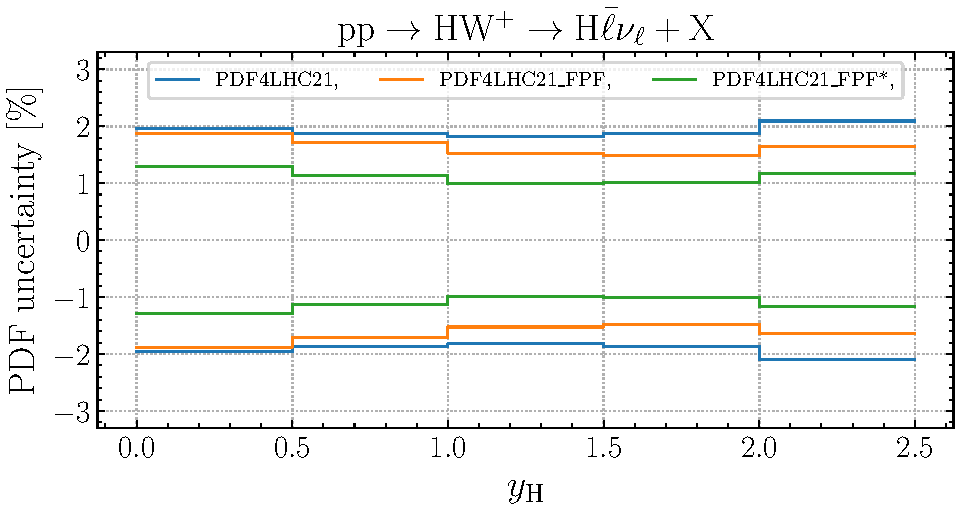
\includegraphics[width=0.49\textwidth]{plots/LHCpheno/NNPDF_HWP_14TEV_40_PHENO-global-pdf4lhc21.pdf}
	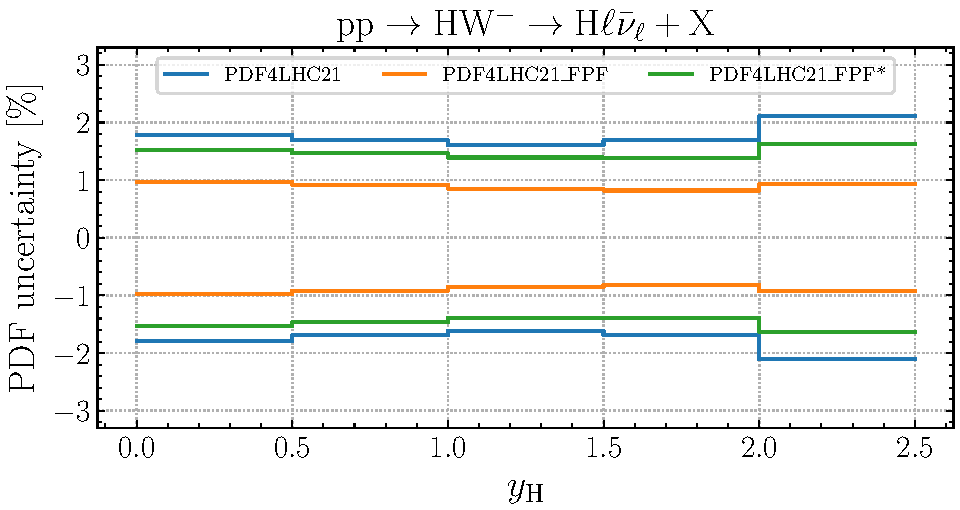
\includegraphics[width=0.49\textwidth]{plots/LHCpheno/NNPDF_HWM_14TEV_40_PHENO-global-pdf4lhc21.pdf}
	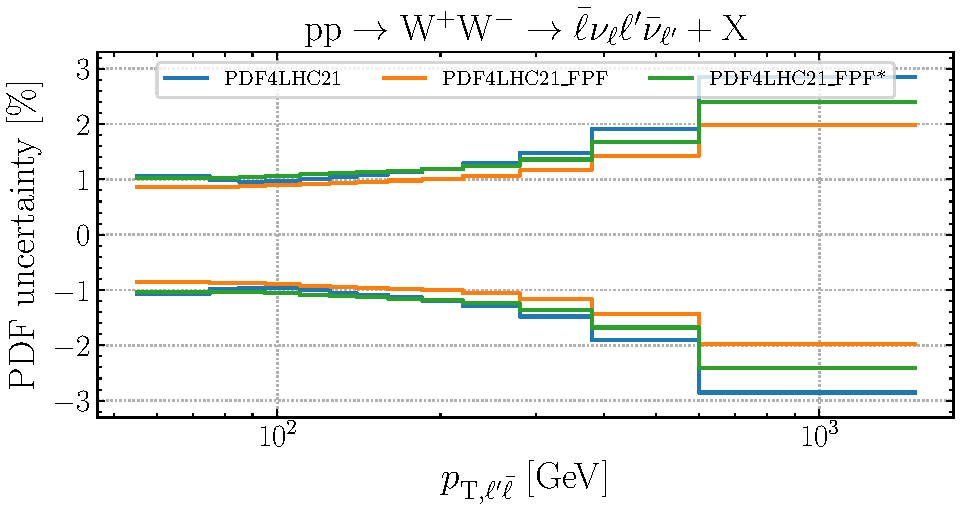
\includegraphics[width=0.49\textwidth]{plots/LHCpheno/NNPDF_WPWM_14TEV_40_PHENO-global-pdf4lhc21.pdf}
	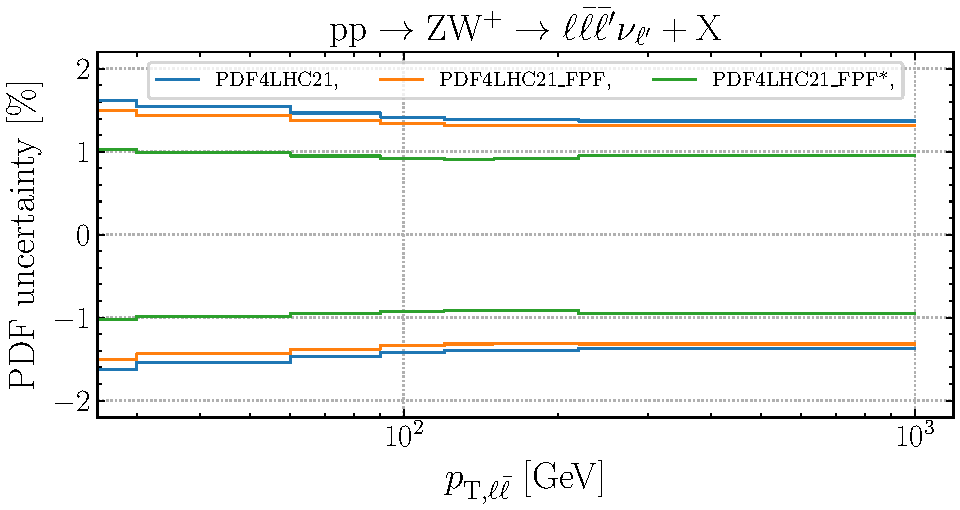
\includegraphics[width=0.49\textwidth]{plots/LHCpheno/NNPDF_WPZ_14TEV_40_PHENO-global-pdf4lhc21.pdf}
	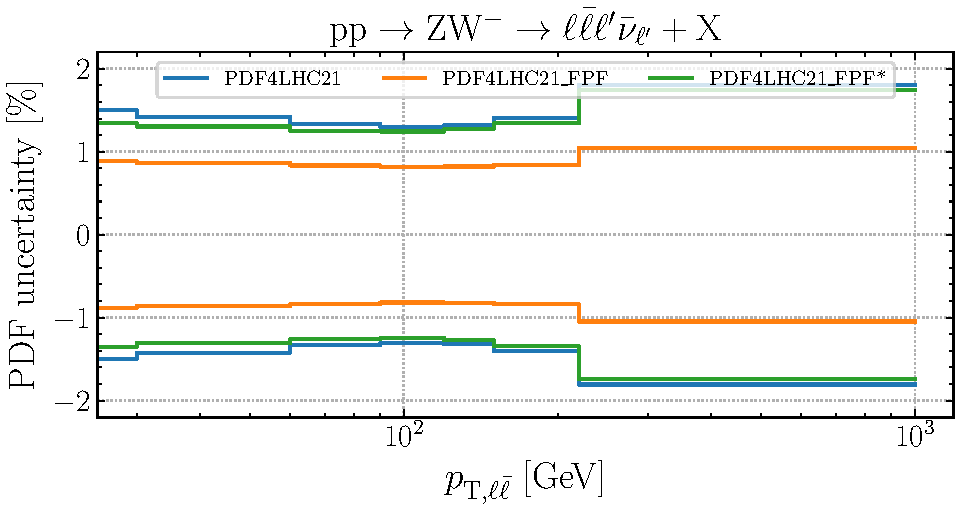
\includegraphics[width=0.49\textwidth]{plots/LHCpheno/NNPDF_WMZ_14TEV_40_PHENO-global-pdf4lhc21.pdf}
	\caption{
		Same as Fig.~\ref{fig:NNPDF40_pheno_differential} but with PDF4LHC21.
	}
	\label{fig:PDF4LHC21_pheno_differential}
\end{figure}
%%%%%%%%%%%%%%%%%%%%%%%%%%%%%%%%%%%%%%%%%%%%%%%%%%%%%%%%%%%%%%%%%%%%%%%%

Inspection of Figs.~\ref{fig:NNPDF40_pheno_integrated} and~\ref{fig:NNPDF40_pheno_differential}
quantifies the potential of neutrino structure function measurements at the LHC
to improve theoretical predictions for electroweak and high-scale processes at the HL-LHC.
%
Concerning first the fiducial integrated cross-sections, a reduction of PDF
uncertainties is observed for all processes,
including for $W^+$ production relevant for $m_W$ measurements, and its specific  magnitude depends
on the underlying scattering reaction.
%
This finding also applies for Higgs associated production with vector bosons and in vector-boson-scattering,
with for example
PDF uncertainties in $hW^+$ reduced by up to a factor two thanks to the FPF measurements.
%
Similar remarks apply to the diboson cross-sections, with in this case the largest
improvement observed for $ZW^+$ channel.
%
Reassuringly, LHC predictions based on the fits with FPF pseudo-data are stable
upon the inclusion of the experimental systematic uncertainties in the fit.

In the case of the differential cross-sections shown in Fig.~\ref{fig:NNPDF40_pheno_differential},
we observe how the impact of the FPF structure functions on LHC observables depends
on the hard-scattering scale.
%
For instance, searches for heavy-resonances in the high-mass tail of the Drell-Yan
distributions are going to be improved by FPF data.
%
The same applies for diboson prediction, and in the case of the $ZW^+$ channel we observe
an improvement spatially in the low $p_{T,\ell\bar{\ell}}$ region.
%
For the Higgs production processes, the PDF uncertainty in the theory predictions is relatively
stable as a function of the rapidity.
%
The effects of accounting for systematic uncertainties in the fit are somewhat more visible
here as compared to the inclusive cross-sections, indicating that they affect mostly
the tails, rather than the bulk, of the distributions, and in particular the large-$x$
behaviour of the PDFs.



The studies presented in this section provide only a first glimpse of the potential
of neutrino DIS measurements at the LHC to inform predictions for high-$p_T$ processes.


